% Dataset stats: CMD-ISI
\begin{figure}[ht]
\captionsetup[subfigure]{labelformat=empty}
\begin{center}
\subfloat[adi]{\label{fig:dstats:CMD:ISI:adi}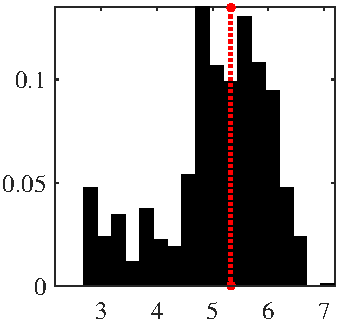
\includegraphics[scale=1]{dstats/CMD-adi-ISI.pdf}} \hspace{0.5cm} 
\subfloat[rupaka]{\label{fig:dstats:CMD:ISI:rupaka}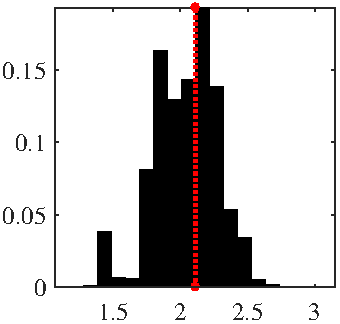
\includegraphics[scale=1]{dstats/CMD-rupaka-ISI.pdf}} \\ 
\subfloat[mishraChapu]{\label{fig:dstats:CMD:ISI:mishraChapu}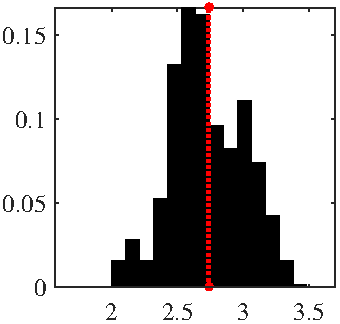
\includegraphics[scale=1]{dstats/CMD-mishraChapu-ISI.pdf}} \hspace{0.5cm} 
\subfloat[khandaChapu]{\label{fig:dstats:CMD:ISI:khandaChapu}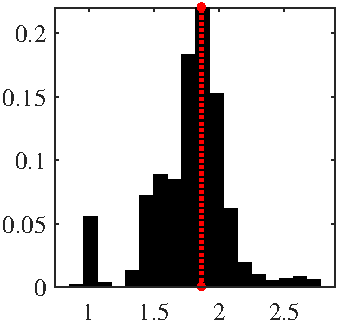
\includegraphics[scale=1]{dstats/CMD-khandaChapu-ISI.pdf}} \\ 
\caption[CMD-ISI]{CMD-ISI}\label{fig:dstats:CMD:ISI}
\end{center}
\end{figure}
%
%
% Dataset stats: CMDf-ISI
\begin{figure}[ht]
\captionsetup[subfigure]{labelformat=empty}
\begin{center}
\subfloat[adi]{\label{fig:dstats:CMDf:ISI:adi}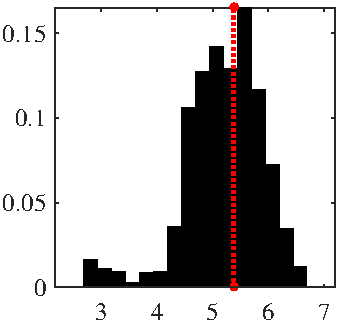
\includegraphics[scale=1]{dstats/CMDf-adi-ISI.pdf}} \hspace{0.5cm} 
\subfloat[rupaka]{\label{fig:dstats:CMDf:ISI:rupaka}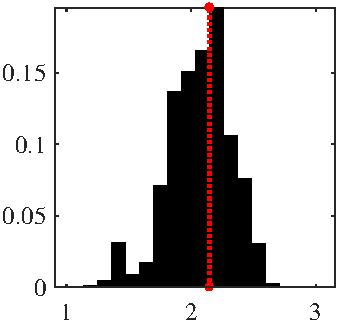
\includegraphics[scale=1]{dstats/CMDf-rupaka-ISI.pdf}} \\ 
\subfloat[mishraChapu]{\label{fig:dstats:CMDf:ISI:mishraChapu}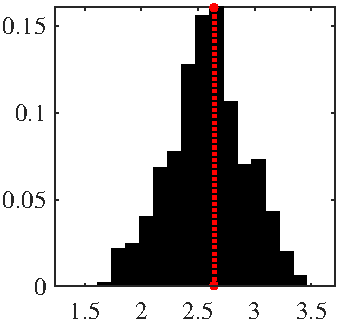
\includegraphics[scale=1]{dstats/CMDf-mishraChapu-ISI.pdf}} \hspace{0.5cm} 
\subfloat[khandaChapu]{\label{fig:dstats:CMDf:ISI:khandaChapu}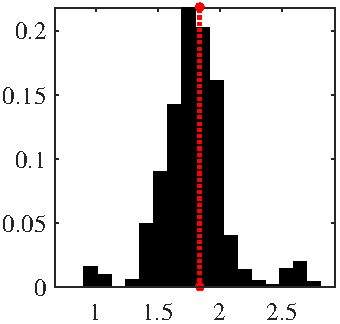
\includegraphics[scale=1]{dstats/CMDf-khandaChapu-ISI.pdf}} \\ 
\caption[CMDf-ISI]{CMDf-ISI}\label{fig:dstats:CMDf:ISI}
\end{center}
\end{figure}
%
%
% Dataset stats: HMDf-ISI
\begin{figure}[ht]
\captionsetup[subfigure]{labelformat=empty}
\begin{center}
\subfloat[teen]{\label{fig:dstats:HMDf:ISI:teen}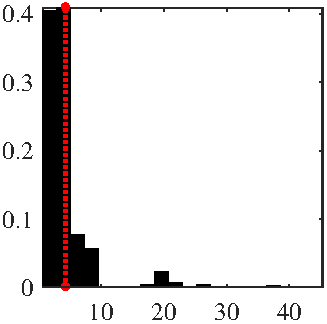
\includegraphics[scale=1]{dstats/HMDf-teen-ISI.pdf}} \hspace{0.5cm} 
\subfloat[ek]{\label{fig:dstats:HMDf:ISI:ek}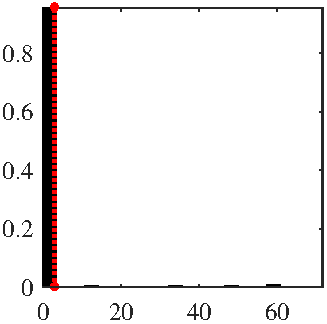
\includegraphics[scale=1]{dstats/HMDf-ek-ISI.pdf}} \\ 
\subfloat[jhap]{\label{fig:dstats:HMDf:ISI:jhap}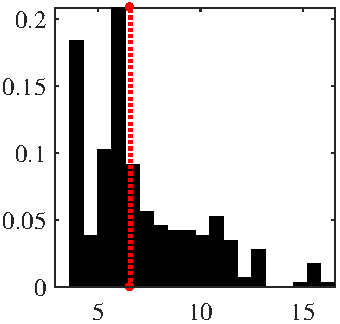
\includegraphics[scale=1]{dstats/HMDf-jhap-ISI.pdf}} \hspace{0.5cm} 
\subfloat[rupak]{\label{fig:dstats:HMDf:ISI:rupak}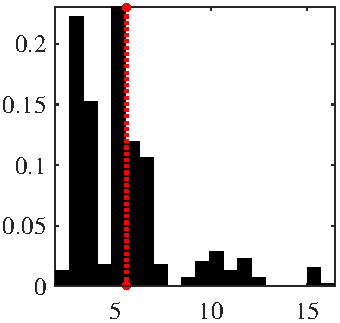
\includegraphics[scale=1]{dstats/HMDf-rupak-ISI.pdf}} \\ 
\caption[HMDf-ISI]{HMDf-ISI}\label{fig:dstats:HMDf:ISI}
\end{center}
\end{figure}
%
%
% Dataset stats: HMDl-ISI
\begin{figure}[ht]
\captionsetup[subfigure]{labelformat=empty}
\begin{center}
\subfloat[teen]{\label{fig:dstats:HMDl:ISI:teen}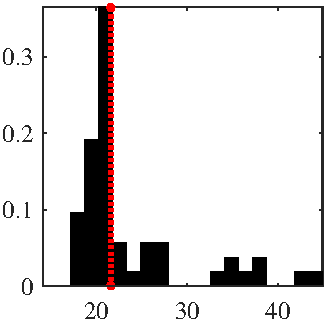
\includegraphics[scale=1]{dstats/HMDl-teen-ISI.pdf}} \hspace{0.5cm} 
\subfloat[ek]{\label{fig:dstats:HMDl:ISI:ek}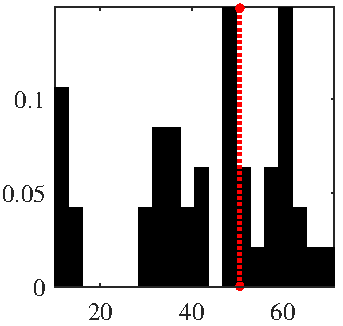
\includegraphics[scale=1]{dstats/HMDl-ek-ISI.pdf}} \\ 
\subfloat[jhap]{\label{fig:dstats:HMDl:ISI:jhap}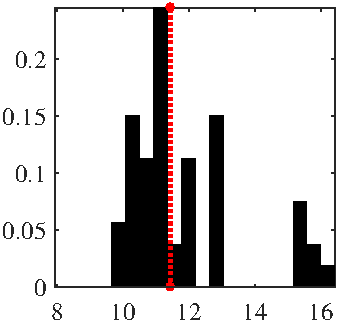
\includegraphics[scale=1]{dstats/HMDl-jhap-ISI.pdf}} \hspace{0.5cm} 
\subfloat[rupak]{\label{fig:dstats:HMDl:ISI:rupak}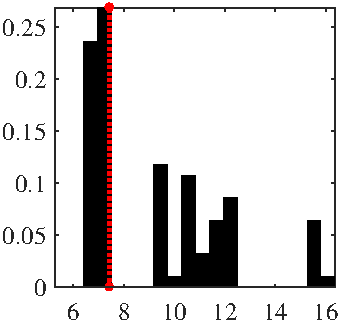
\includegraphics[scale=1]{dstats/HMDl-rupak-ISI.pdf}} \\ 
\caption[HMDl-ISI]{HMDl-ISI}\label{fig:dstats:HMDl:ISI}
\end{center}
\end{figure}
%
%
% Dataset stats: HMDs-ISI
\begin{figure}[ht]
\captionsetup[subfigure]{labelformat=empty}
\begin{center}
\subfloat[teen]{\label{fig:dstats:HMDs:ISI:teen}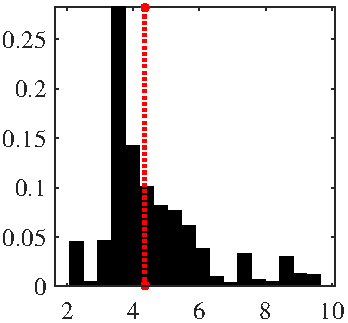
\includegraphics[scale=1]{dstats/HMDs-teen-ISI.pdf}} \hspace{0.5cm} 
\subfloat[ek]{\label{fig:dstats:HMDs:ISI:ek}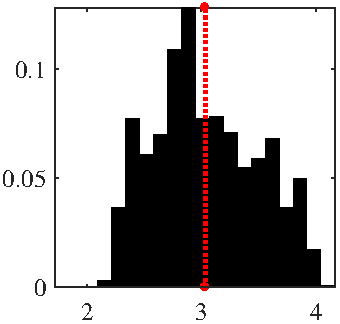
\includegraphics[scale=1]{dstats/HMDs-ek-ISI.pdf}} \\ 
\subfloat[jhap]{\label{fig:dstats:HMDs:ISI:jhap}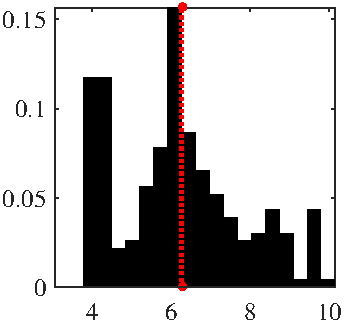
\includegraphics[scale=1]{dstats/HMDs-jhap-ISI.pdf}} \hspace{0.5cm} 
\subfloat[rupak]{\label{fig:dstats:HMDs:ISI:rupak}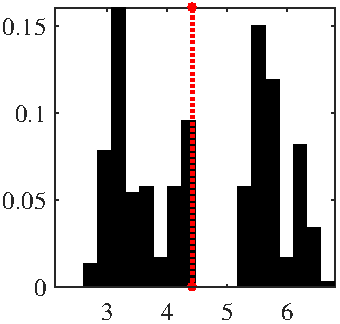
\includegraphics[scale=1]{dstats/HMDs-rupak-ISI.pdf}} \\ 
\caption[HMDs-ISI]{HMDs-ISI}\label{fig:dstats:HMDs:ISI}
\end{center}
\end{figure}
%
%
